\section{Tir planeta okoli sonca}

Rešujemo sistem navadnih diferencialnih enačb, ki predstavljajo gibalno enačbo gibanja planeta okoli nepomičnega sonca v ravnini
\begin{equation}
    \vec{r} = -G \frac{M\,\vec{r}}{r^3},
\end{equation}
kjer je $\vec{r}$ vektor pospeškov. Za numerično obravnavo zapišemo sistem enačb v obliki $\frac{dy}{dt} = f(x,y)$, ki ga je mogoče ``integrirati''
\begin{align}
    \dot{x} &= v_x \\ \nonumber
    \dot{y} &= v_y \\ \nonumber
    \ddot{x} &= \frac{x}{(x^2+y^2)^{3/2}} \\ \nonumber
    \ddot{y} &= \frac{y}{(x^2+y^2)^{3/2}}, \\ \nonumber
\end{align}
kjer predpostavimo, da je $G\,M=0$ in obravnavamo sistem brezdimenzijsko. Pri tem moramo določiti začetne pogoje
\begin{equation}
    \vec{y_0} = (x_0, y_0, v_{x0},v_{y0}).
\end{equation}

Za reševanje uporabljamo tako metode, vgrajene v \texttt{scipy.integrate.solve\_ivp}, kot tudi lastno implementirane: eksplicitno Euler-jevo metodo, Runge-Kutta metodo 4. reda in simplektično Verlet-ovo metodo.

Na spodnji sliki je prikazano, kako se obnesejo metode pri različnih začetnih pogojih $\vec{y_0}=(1,0,0,v_{0})$. Poznamo značilne tire:
\begin{itemize}
    \item $v_0<1$ tir je elipsa
    \item $v_0=1$ tir je krožnica
    \item $1<v_0<\sqrt{2}$ tir je elipsa
    \item $v_0=\sqrt{2}$ tir je parabola
    \item $v_0>\sqrt{2}$ tir je hiperbola
\end{itemize}
Presenetljivo je, da se, poleg Verleta izredno dobro obnese tudi lastna implementacija Runge-Kutta 4.reda, očitno bolje od \textit{RK45} v \texttt{solve\_ivp}, kar bomo analizirali v sledečem delu. Euler-jeva metoda ob večjem koraku (pričakovano) hitro odpove, velja tudi poudariti, da imajo metode iz \texttt{solve\_ivp} možnost avtomatskega prilagajanja časovnega koraka, vendar so izračuni izvedeni pri konstantnem koraku.

\begin{figure}[ht]
    \centering
    \begin{subfigure}{0.49\textwidth}
        \centering
        \includegraphics[width=\linewidth]{1.nal_slike/v0_0.25.pdf}
        \caption{}
    \end{subfigure}
    \begin{subfigure}{0.49\textwidth}
        \centering
        \includegraphics[width=\linewidth]{1.nal_slike/v0_0.5.pdf}
        \caption{}
    \end{subfigure}
    \begin{subfigure}{0.49\textwidth}
        \centering
        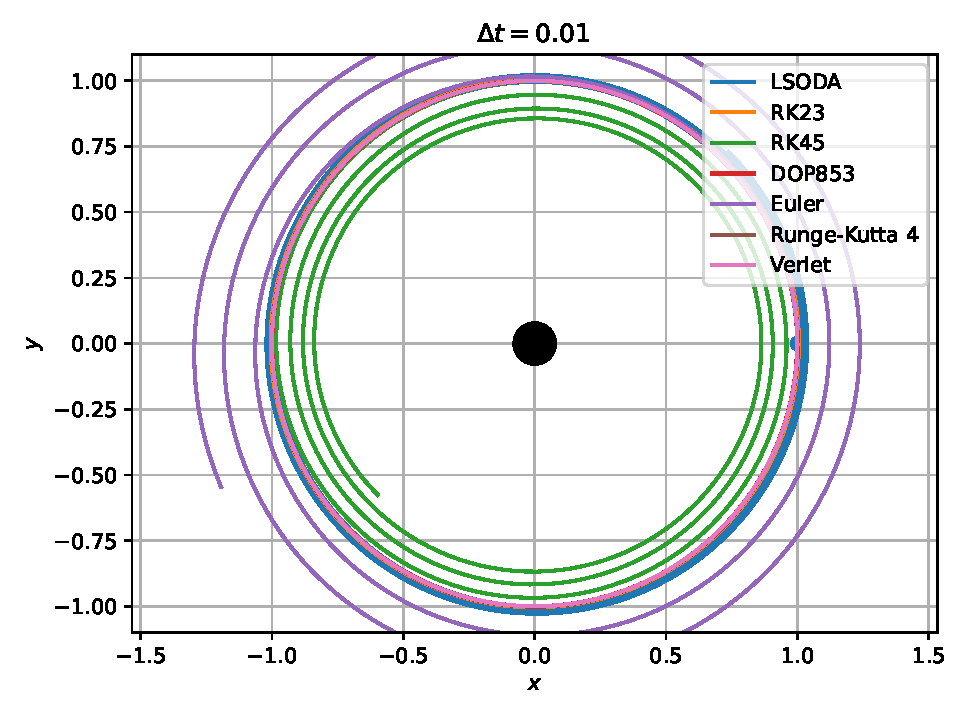
\includegraphics[width=\linewidth]{1.nal_slike/v0_1.pdf}
        \caption{}
    \end{subfigure}
    \begin{subfigure}{0.49\textwidth}
        \centering
        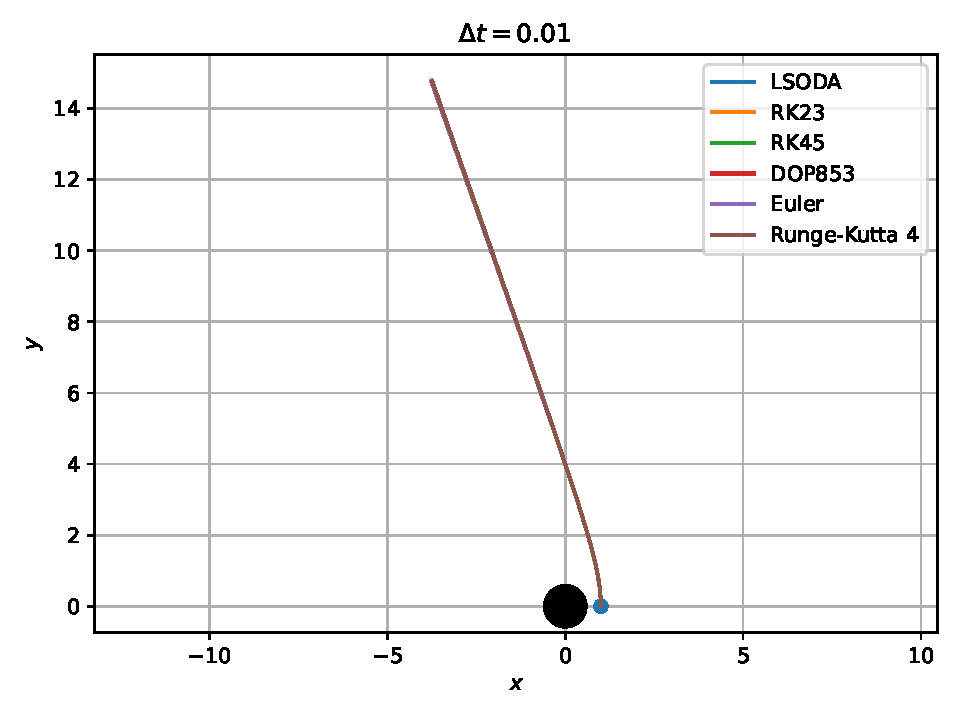
\includegraphics[width=\linewidth]{1.nal_slike/v0_2.pdf}
        \caption{}
    \end{subfigure}
    \caption[short]{Trajektorije planeta pri začetni hitrosti $v_0$ (a) 0.25, (b) 0.5, (c) 1 in (d) 2}
\end{figure}

Na spodnji sliki vidimo, kako se Euler oddaljuje od prave rešitve. Sicer mi pa ni jasno, zakaj sta komponenti hitrosti pri RK45 ravno obratni kot pri lastni implementaciji, saj je lega pravilna! V vseh primerih je uporabljen korak $\Delta t=0.001$~s, razen če je napisano drugače.

\begin{figure}[H]
    \centering
    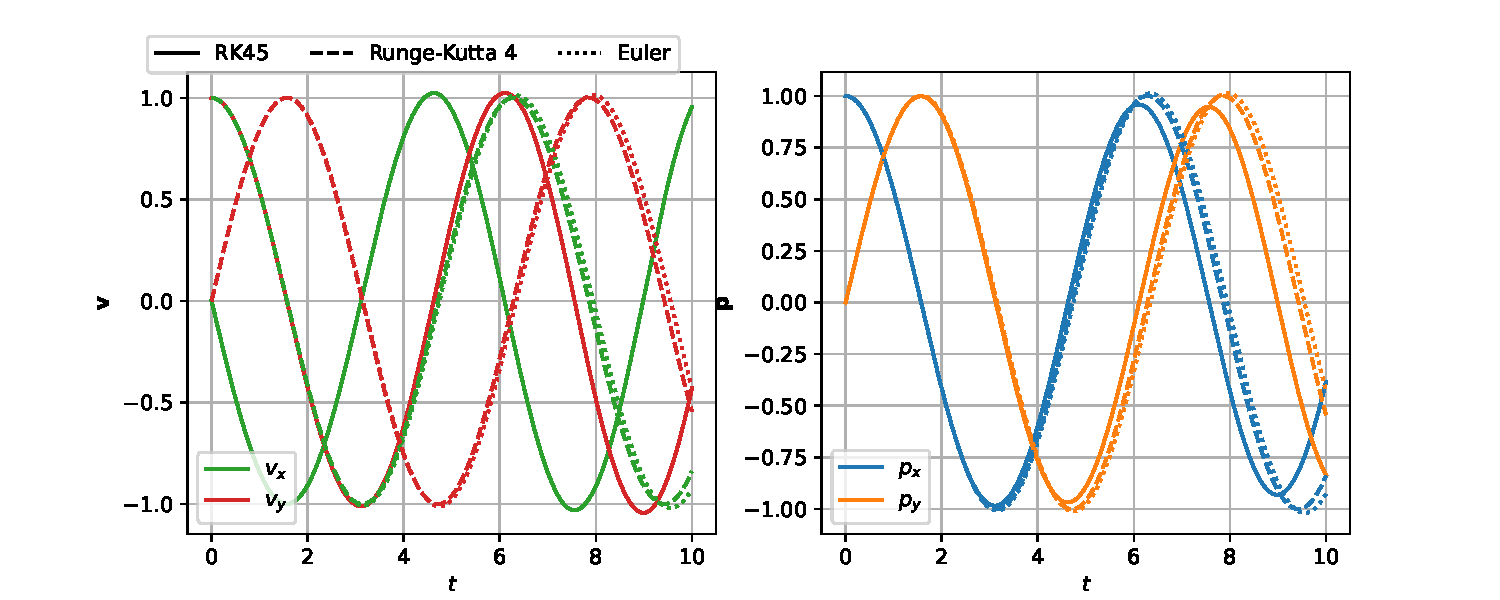
\includegraphics[width=\linewidth]{1.nal_slike/potek_v_p_v0_1.pdf}
    \caption[short]{Potek hitrosti in lege po komponentah za primer $v_0=1$}
\end{figure}

Na spodnji sliki se bolje vidi, kako nekatere metode slabo ohranjajo periodo. Čeprav gre za krožno gibanje, lahko iz najboljših približkov vidimo očitno periodičnost. DOP853 ima oscilacije lege, ki pa niso posledica glavnega gibanja planeta.

\begin{figure}[H]
    \centering
    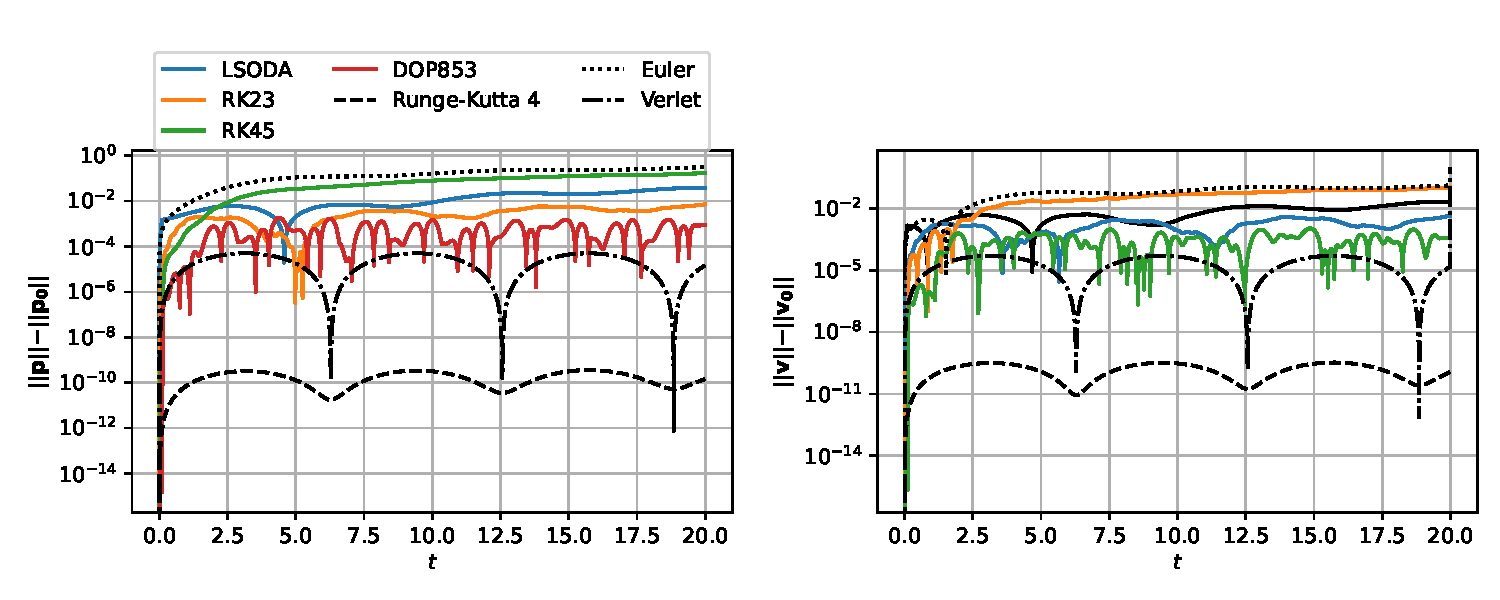
\includegraphics[width=\linewidth]{1.nal_slike/potek_abs_p_v_v0_1.pdf}
    \caption[short]{Potek absolutnih hitrosti in lege za $v_0=1$}
\end{figure}

Pri tem spremljamo tudi potek vrtilne količine okoli z-osi, energije in komponent Runge-Lenz-ovega vektorja. Vrtilna količina se pričakovano ohranja, prav tako energija, vendar je popolnoma konstantna vrednost SUMLJIVA! Runge-Lenz-ov vektor ima tudi ČUDNO velika nihanja. Skok vrilne količine pri Verletu je nerelevanten in je posledica aproksimacije hitrosti iz pomikov, ki na robu ni mogoča (po centralni diferenčni shemi). Ostale metode imajo večje vrednosti, vendar večina manjša nihanja. Ponovno se odlično izkaže lastna implementacija Runge-Kutte, ki ima najnižje vrednosti brez prenihavanj.

\begin{figure}[H]
    \centering
    \begin{subfigure}{0.49\textwidth}
        \centering
        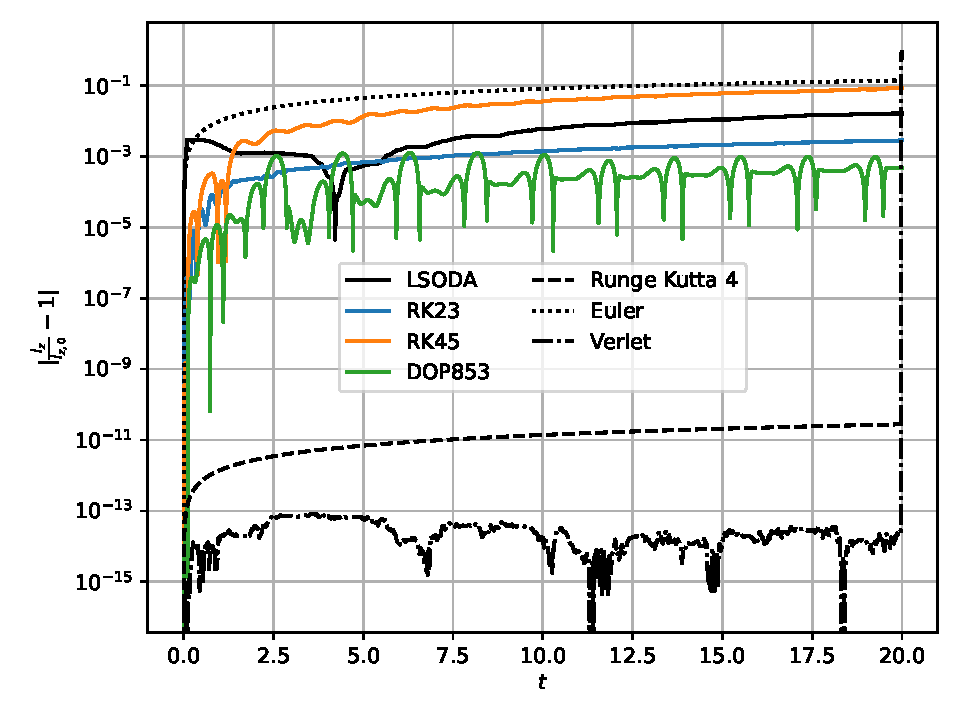
\includegraphics[width=\linewidth]{1.nal_slike/potek_lz_v0_1.pdf}
        \caption{}
    \end{subfigure}
    \begin{subfigure}{0.49\linewidth}
        \centering
        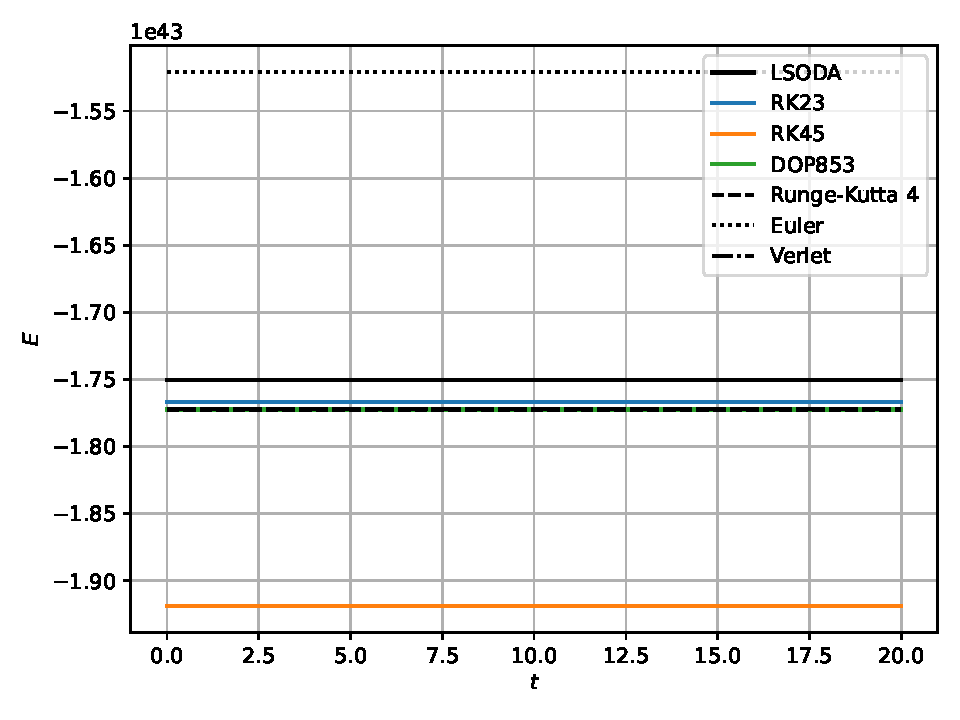
\includegraphics[width=\linewidth]{1.nal_slike/E_v0_1.pdf}
        \caption{}
    \end{subfigure}
    \begin{subfigure}{0.49\linewidth}
        \centering
        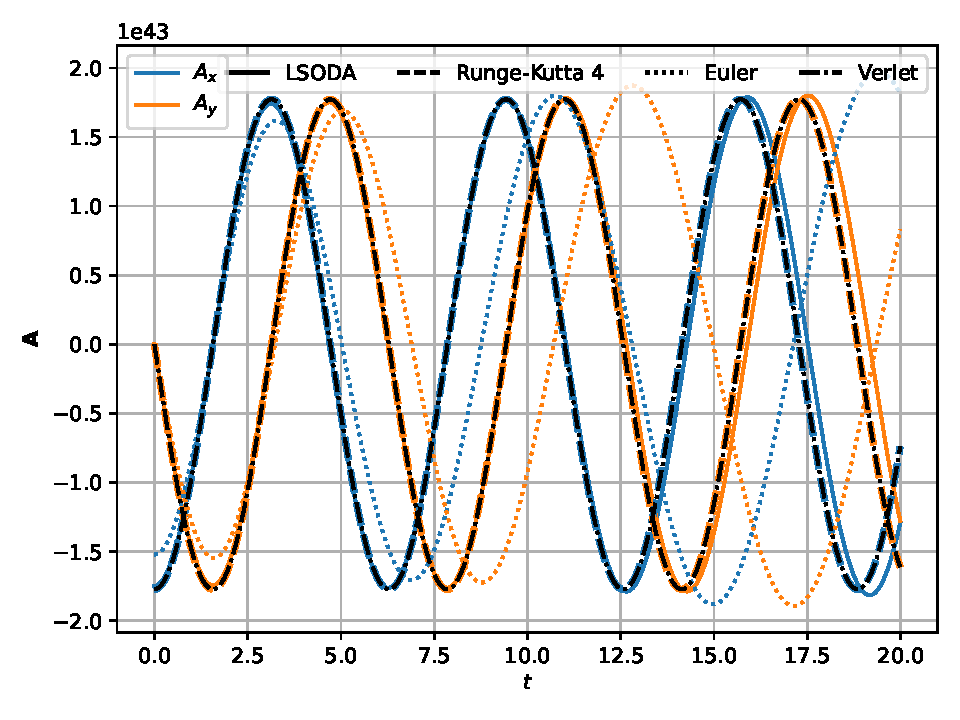
\includegraphics[width=\linewidth]{1.nal_slike/potek_A_v0_1.pdf}
        \caption{}
    \end{subfigure}
    \caption[short]{Potek (a) vrtilne količine, (b) energije in (c) Runge-Lenz vektorja pri $v_0=1$}
\end{figure}

Spodaj so prikazane enake stveri, vendar tokrat za elipsasti tir ($v_0=0.5$). Opažanja so enaka kot zgoraj.

\begin{figure}[H]
    \centering
    \begin{subfigure}{0.49\textwidth}
        \centering
        \includegraphics[width=\linewidth]{1.nal_slike/potek_lz_v0_0.5.pdf}
        \caption{}
    \end{subfigure}
    \begin{subfigure}{0.49\linewidth}
        \centering
        \includegraphics[width=\linewidth]{1.nal_slike/E_v0_0.5.pdf}
        \caption{}
    \end{subfigure}
    \begin{subfigure}{0.49\linewidth}
        \centering
        \includegraphics[width=\linewidth]{1.nal_slike/potek_A_v0_0.5.pdf}
        \caption{}
    \end{subfigure}
    \caption[short]{Potek (a) vrtilne količine, (b) energije in (c) Runge-Lenz vektorja pri $v_0=0.5$}
\end{figure}

Prikažem še poteke hitrosti in pomikov, od koder lahko vidimo periodo in kako dobro jo katera metoda ohranja. Lastna implementacija Verlet in Runge-Kutta 4 se takorekoč prekrivata, razen pri  $v_0=0.1$, kjer Runge-Kutta že odpove. Pri spodnjih dveh grafih je časovni korak dodatno zmanjšan na $\Delta t = 0.0001$. Tudo DOP853 se dobro izkaže, zanimivo pa je, da je RK23 celo bolj uspešna od RK45! Tudi od LSODA se pričakoval več, glede na to, da je implementirana tudi za toge sisteme.

\begin{figure}[ht]
    \centering
    \begin{subfigure}{0.49\textwidth}
        \centering
        \includegraphics[width=\linewidth]{1.nal_slike/potek_abs_p_v_v0_0.5.pdf}
        \caption{}
    \end{subfigure}
    \begin{subfigure}{0.49\linewidth}
        \centering
        \includegraphics[width=\linewidth]{1.nal_slike/potek_abs_p_v_v0_0.25.pdf}
        \caption{}
    \end{subfigure}
    \begin{subfigure}{0.49\linewidth}
        \centering
        \includegraphics[width=\linewidth]{1.nal_slike/potek_abs_p_v_v0_0.2.pdf}
        \caption{}
    \end{subfigure}
    \begin{subfigure}{0.49\linewidth}
        \centering
        \includegraphics[width=\linewidth]{1.nal_slike/potek_abs_p_v_v0_0.1.pdf}
        \caption{}
    \end{subfigure}
    \caption[short]{Potek absolutnih hitrosti in lege za $v_0$ (a) 0.5, (b) 0.25, (c) 0.2 in (d) 0.1}
\end{figure}

Za bolj natančno določitev časa prehoda sem se odločil za spektralno analizo, saj lahko od tam sklepamo o periodičnosti tira. In res se izkaže tako, še zelo dobro lahko na tak način določimo tudi preostale časovne komponente. Na spodnji sliki je prikazan tako FFT v 2D, kot na absolutnih vrednostih lege in hitrosti. Pri $v_0=1$ lahko iz vseh grafov razberemo ekstrem okoli časa 650, kar predstavlja obhodni čas, saj
$$
\frac{2\,\pi}{\Delta t} \approx 628,
$$
skala na grafih pa ni množena z $\Delta t$. Čudno mi je, da ima moja Runge-Kutta tako nizke vrednosti! V komponentni obliki se se sicer vrednosti Verlet, Runge-Kutta 4 in DOP853 takorekoč prekrivajo v legah in hitrostih, zelo blizu sta tudi RK23 in LSODA, za napako pri RK45 pa nimam pojasnila!

\begin{figure}[ht]
    \centering
    \begin{subfigure}{0.49\textwidth}
        \centering
        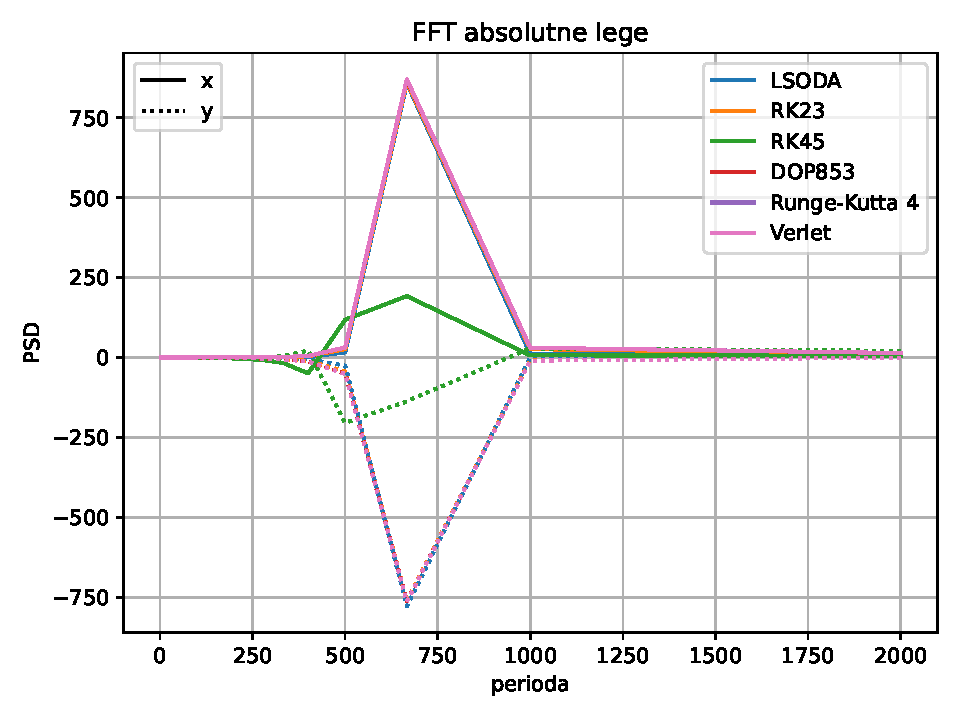
\includegraphics[width=\linewidth]{1.nal_slike/fft/fft_lege_v0_1.pdf}
    \end{subfigure}
    \begin{subfigure}{0.49\textwidth}
        \centering
        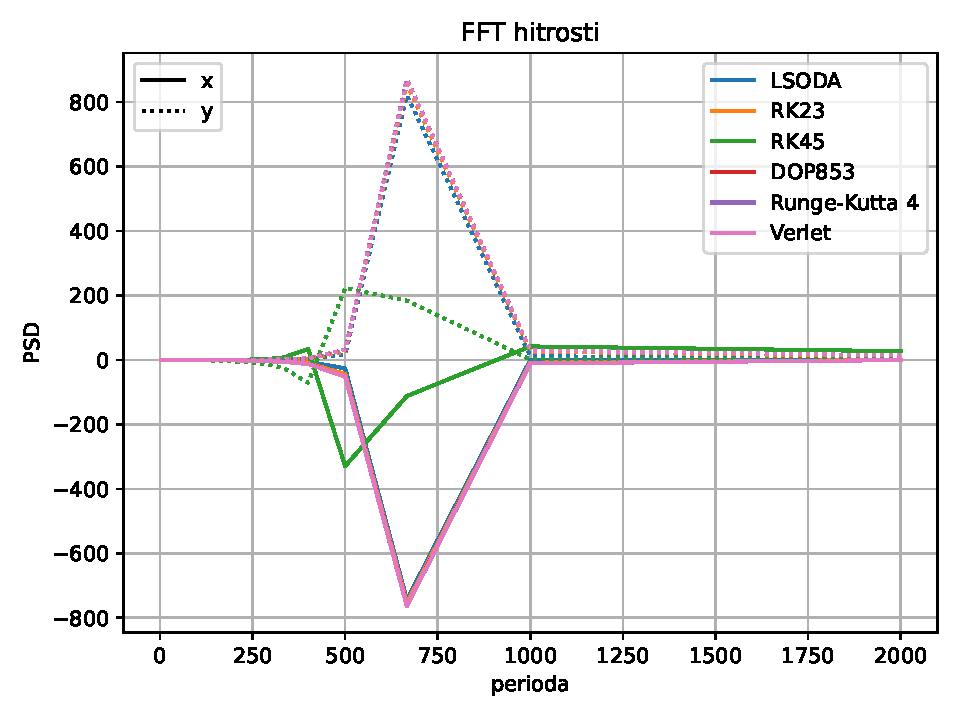
\includegraphics[width=\linewidth]{1.nal_slike/fft/fft_hitr_v0_1.pdf}
    \end{subfigure}
    \begin{subfigure}{0.49\textwidth}
        \centering
        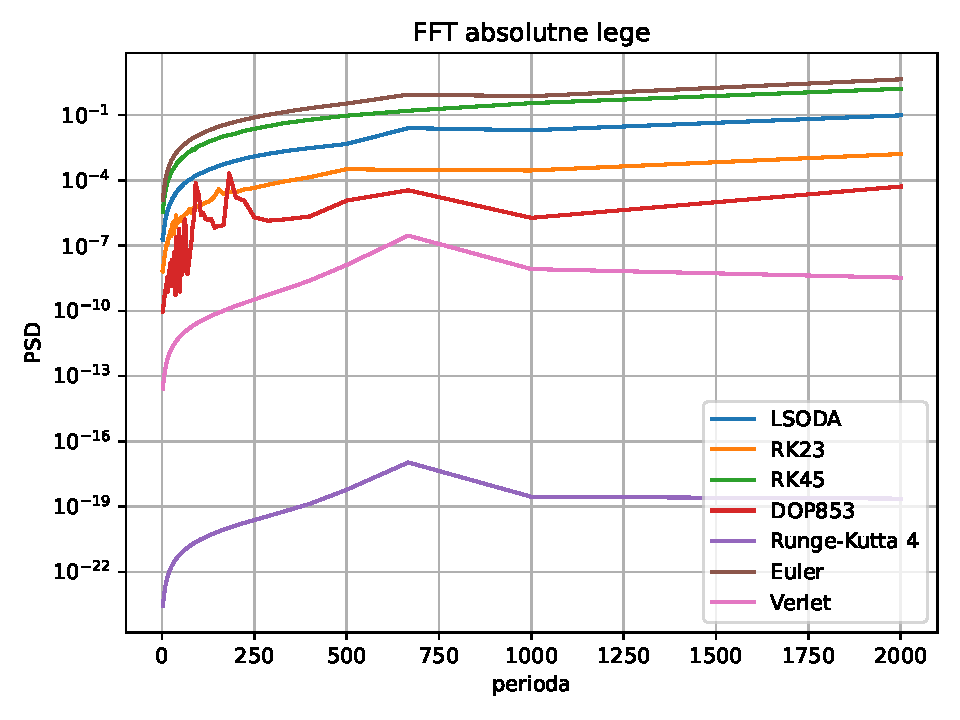
\includegraphics[width=\linewidth]{1.nal_slike/fft/fft_abs_lege_v0_1.pdf}
    \end{subfigure}
    \begin{subfigure}{0.49\textwidth}
        \centering
        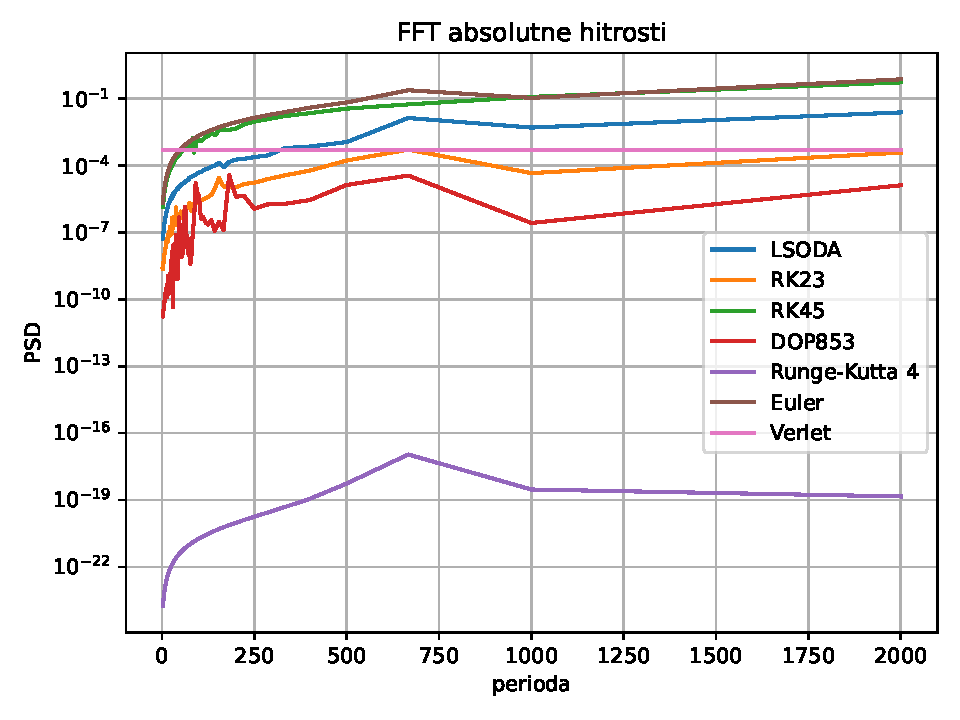
\includegraphics[width=\linewidth]{1.nal_slike/fft/fft_abs_hitr_v0_1.pdf}
    \end{subfigure}
    \caption[short]{FFT rezultatov pri $v_0=1$}
\end{figure}

Pri eliptičnem tiru ne morem tako preprosto izračunati obhodnega časa, vendar je na spodnjih grafih tudi uporabljen drugačen $\Delta t = 0.001$, zato vrednosti niso primerljive. V tem primeru se prekrivata le še moja Verlet in Runge-Kutta, za katera predvidevam, da najbolje popisujeta periodo.

\begin{figure}[H]
    \centering
    \begin{subfigure}{0.49\textwidth}
        \centering
        \includegraphics[width=\linewidth]{1.nal_slike/fft/fft_abs_lege_v0_0.5.pdf}
        \caption{}
    \end{subfigure}
    \begin{subfigure}{0.49\textwidth}
        \centering
        \includegraphics[width=\linewidth]{1.nal_slike/fft/fft_abs_hitr_v0_0.5.pdf}
        \caption{}
    \end{subfigure}
    \caption{FFT (a) oddaljenosti od sonca in (b) absolutne hitrosti pri $v_0=0.5$}
\end{figure}

Poizkusil sem tudi z izredno majhno $v_0$, kjer sem moral tudi dodatno zmanjšati časovni korak, vseeno pa ``pobezljata'' Euler (pričakovano) in LSODA (ne tako pričakovano). Iz trajektorij je razvidno, da le še Verlet in Rung-Kutta 4 zadovoljivo popišeta tir.

\begin{figure}[H]
    \centering
    \begin{subfigure}{0.49\textwidth}
        \centering
        \includegraphics[width=\linewidth]{1.nal_slike/v0_0.15.pdf}
        \caption{}
    \end{subfigure}
    \begin{subfigure}{0.49\textwidth}
        \centering
        \includegraphics[width=\linewidth]{1.nal_slike/fft_abs_lege_v0_0.15.pdf}
        \caption{}
    \end{subfigure}
    \caption{(a) Trajektorija planeta pri $v_0=0.15$ (b) FFT oddaljenosti od sonca}
\end{figure}

\subsection{Tir rakete iz planeta}

Dodal sem še eno telo z razmeroma majhno maso, zato lahko predpostavim, da na tir preostalih dveh teles ne vpliva, pač pa le-ti vplivata nanj. Če ima planet začeno lego $\vec{r}_0=(1,0)$ in $\vec{v}_0=(v_0,0)$ ter naša raketa $\vec{r}_{s0}=(1\cdot10^{-3},0)$ in $\vec{v}_{s0}=(v_{s0},v_0)$. Z majhnim razmikom med planetom in raketo zagotovimo možnost simulacije. 

Dobimo podobne tirnice kot pri prejšnji nalogi, vendar odvisno od razmerje $v_{s0}/v_0$:
\begin{itemize}
    \item $v_{s0}/v_0\approx0$ tir je krožnica (telo pade nazaj na planet ko $v_{s0}=0$)
    \item $0<v_{s0}/v_0<1$ tir je elipsa
    \item $v_{s0}/v_0=1$ tir je parabola
    \item $v_{s0}/v_0>1$ tir je hiperbola
\end{itemize}
Zaradi numeričnih težav je izračune blizu $v_{s0}/v_0=0$ težko izvajati!

\begin{figure}[H]
    \begin{subfigure}{0.49\linewidth}
        \centering
        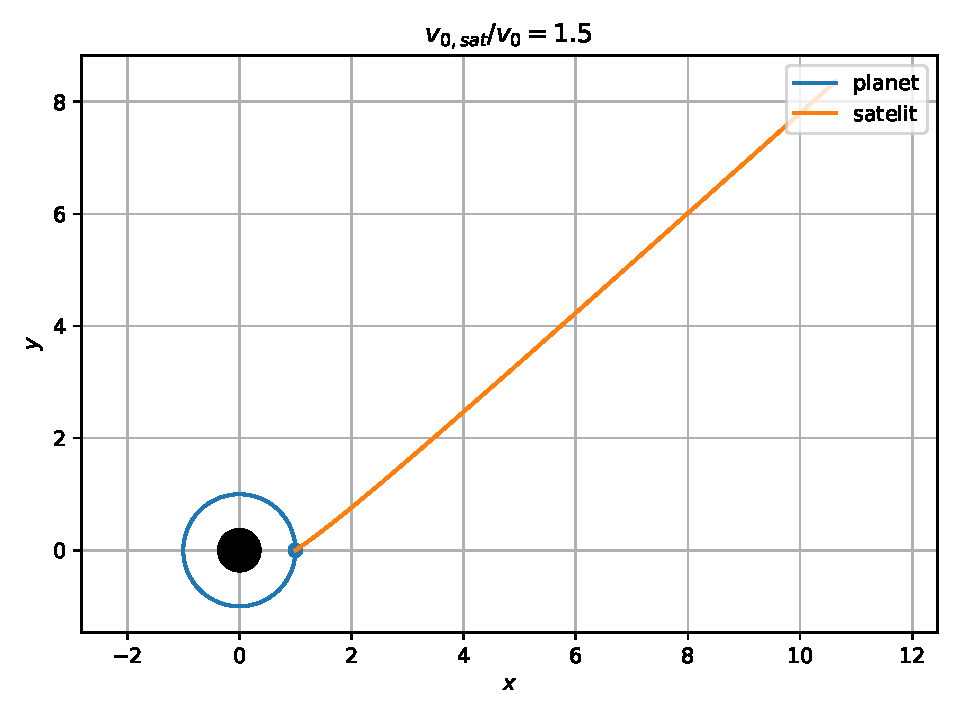
\includegraphics[width=\linewidth]{1.nal_slike/satelit_v1.5.pdf}
        \caption{}
    \end{subfigure}
    \begin{subfigure}{0.49\linewidth}
        \centering
        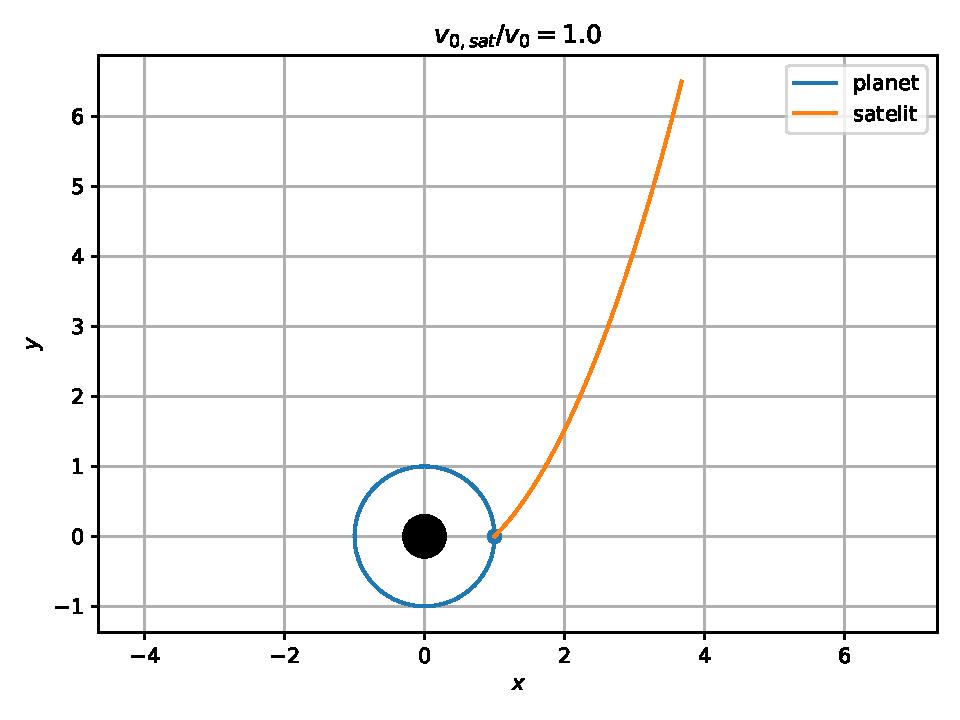
\includegraphics[width=\linewidth]{1.nal_slike/satelit_v1.pdf}
        \caption{}
    \end{subfigure}
    \begin{subfigure}{0.49\linewidth}
        \centering
        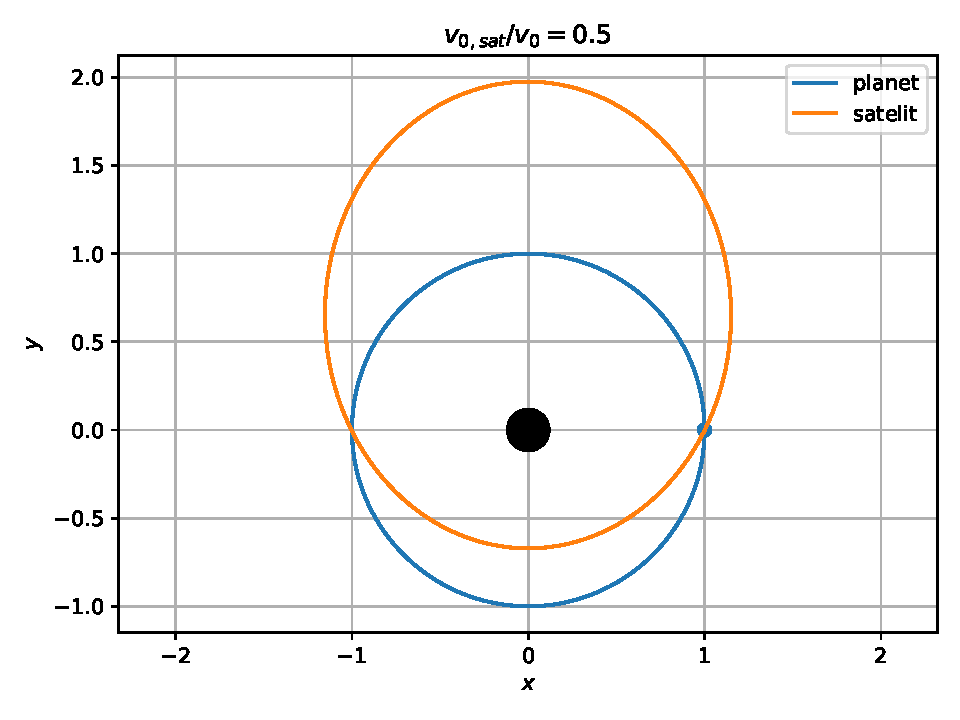
\includegraphics[width=\linewidth]{1.nal_slike/satelit_v0.5.pdf}
        \caption{}
    \end{subfigure}
    \begin{subfigure}{0.49\linewidth}
        \centering
        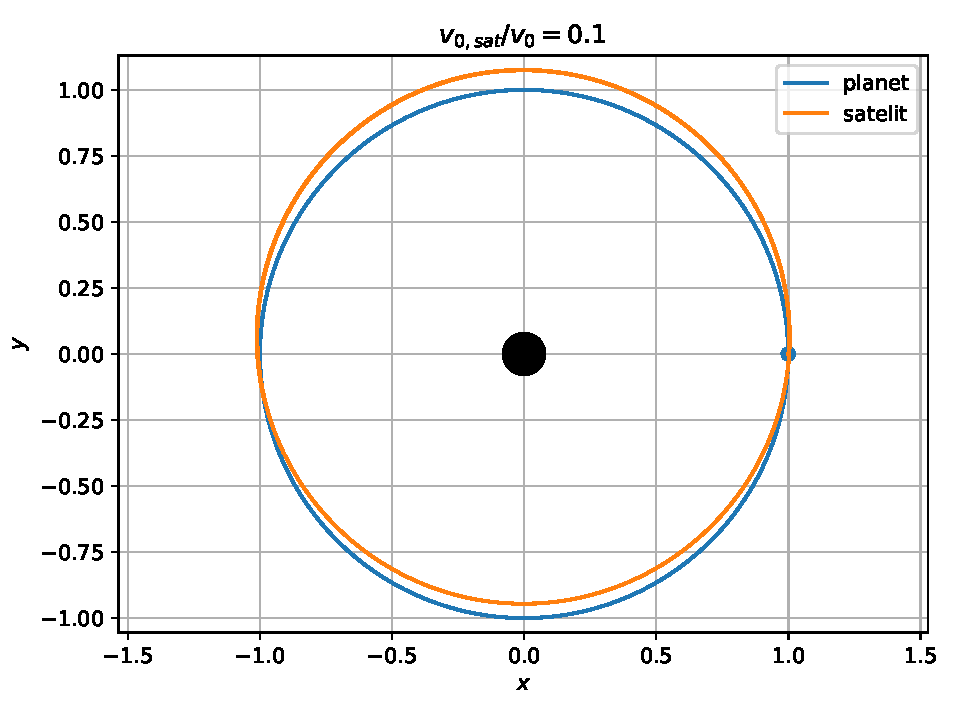
\includegraphics[width=\linewidth]{1.nal_slike/satelit_v0.1.pdf}
        \caption{}
    \end{subfigure}
    \caption[short]{Trajektorija rakete pri izstrelitvi s hitrostjo $v_{s0}$ (a) 1.5, (b) 1, (c) 0.5 in (d) 0.1 pravokotno glede na planet}
\end{figure}

\section{Tir planeta okoli dvojnega sonca}


Če zamenjam sonce z dvojnim soncem, lahko dobim bolj pestre tirnice. Uporabil sem enačbe za \textit{restricted 3-body problem}. Opazim, da je pri razdalji med središčem sonc, ki krožita na razdalji $R_s=0.5$, in planetom $R=1$ tir krožnica (to je tudi 2. Lagrangeeva točka), pri $R=2$ parabola, vmes elipsa in pri $R>2$ hiperbola. Pri $R<1$ gibanje postane nestabilno in navsezadnje planet pobegne iz polja sonc. Prav tako se to zgodi pri spremembi razdalj med soncema, takrat se le-ti ne gibata več eno okoli drugega po krožnici, nego po elipsi, kar vpliva tudi na tir planeta, če so začetni pogoji enaki kot v prejšnjih nalogah.

\begin{figure}[ht]
    \centering
    \begin{subfigure}{0.49\linewidth}
        \centering
        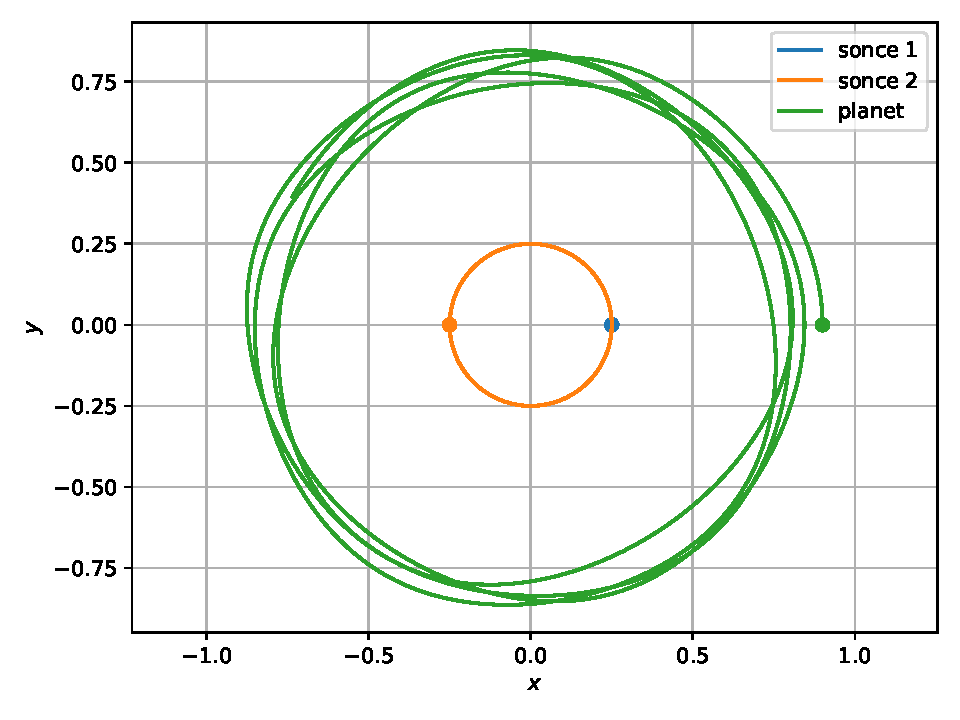
\includegraphics[width=\linewidth]{1.nal_slike/planet_R0.9.pdf}
        \caption{}
    \end{subfigure}
    \begin{subfigure}{0.49\linewidth}
        \centering
        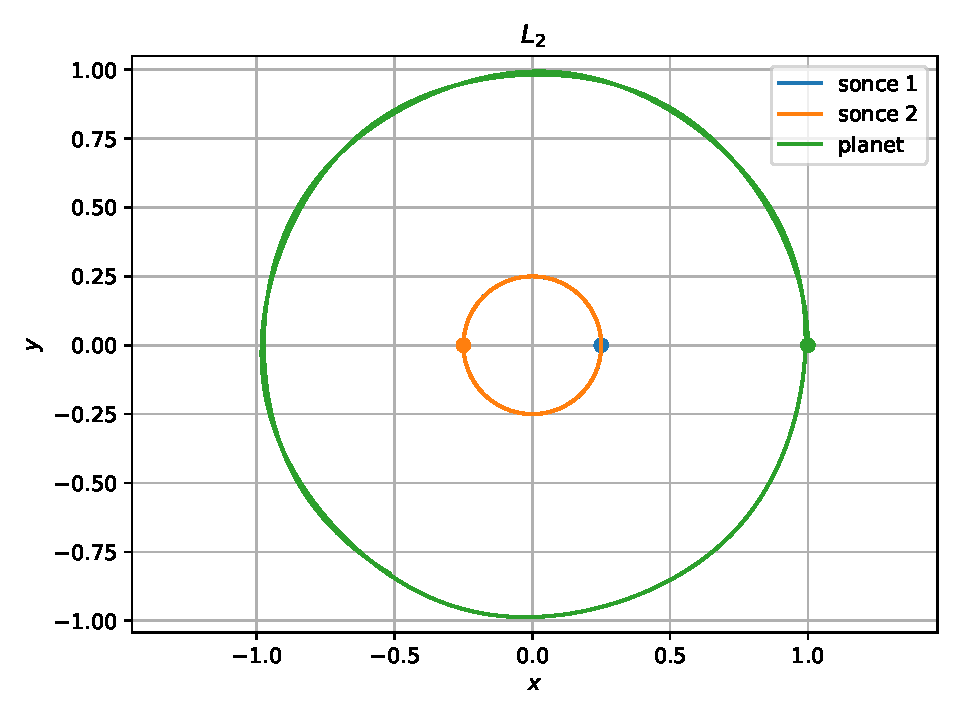
\includegraphics[width=\linewidth]{1.nal_slike/L2}
        \caption{}
    \end{subfigure}
    \begin{subfigure}{0.49\linewidth}
        \centering
        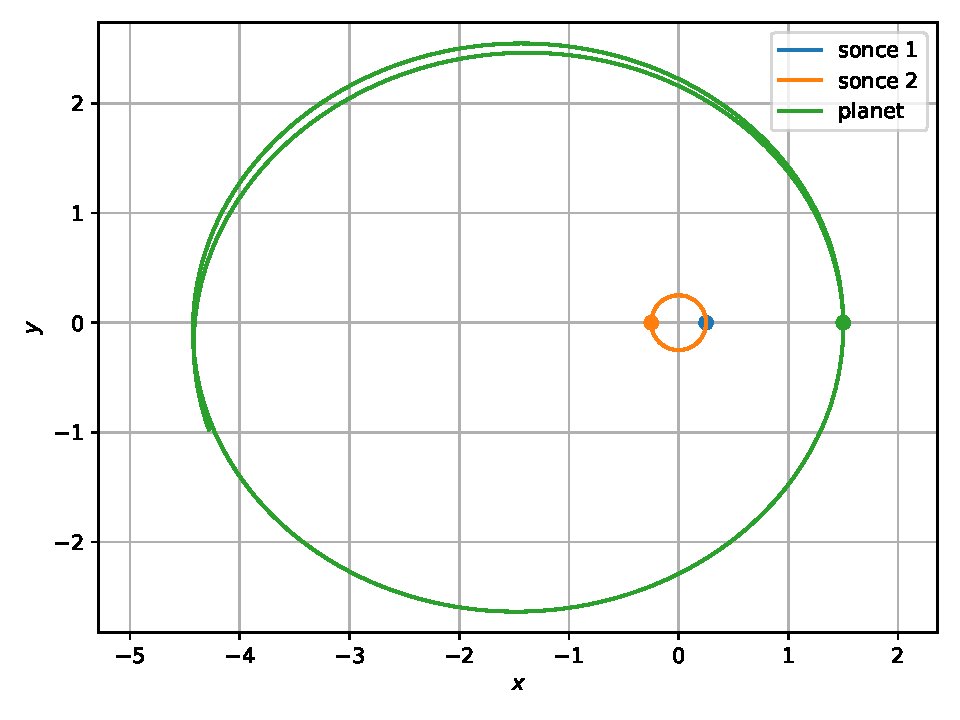
\includegraphics[width=\linewidth]{1.nal_slike/planet_R1.5.pdf}
        \caption{}
    \end{subfigure}
    \begin{subfigure}{0.49\linewidth}
        \centering
        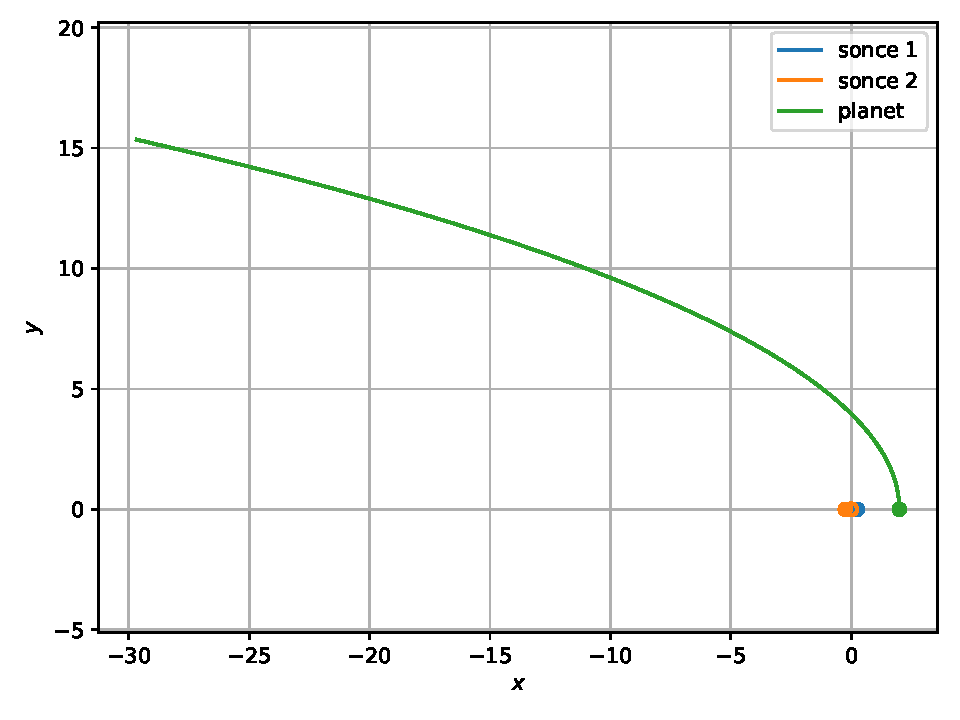
\includegraphics[width=\linewidth]{1.nal_slike/planet_R2.0.pdf}
        \caption{}
    \end{subfigure}
    \caption[short]{Trajektorija planeta na razdalji (a) 0.9, (b) 1, (c) 1.5 in (d) 2 od središča kroženja dvojnega sonca}
\end{figure}

Lahko si pa privoščim, in spremenim začetne pogoje tako, da dobim zanimive orbite,ki so prisotne predvsem okoli Lagrangeeve točke $L_3$, $L_1$ in $L_2$ sta manj zanimivi. Na sliki je prikazana točka L3, ko sonci krožita eno okoli drugega na razdalji $R_s=0.5$ in pri začetnih pogojih lege na razdalji $R=R_s$ in pod kotom $\phi = \pi/2$ ter začetni hitrosi planeta, enaki soncema $v_0=\sqrt{2}$.

Še bolj zanimivo je, če spremenim začetni polarni kot $\phi$ in razdaljo med soncema $R_s$, kar je prikazano v priloženih posnetkih \texttt{trajectory\_angle[$\phi$]\_R[$R_s$].mp4}.

Če zmanjšujem $R_s$ postane gibanje nestabilno, pri povečevanju pa je stabilno do večjih vrednosti. Prav tako se je izkazalo, da vodi do stabilnega tira začetni kot $\phi=\pi/4$ in tudi $\pi/5$ v vseh primerih. Pri nekaterih $R_s$ je sistem stabilen tudi v drugačnih začetnih pogojih hitrosti in kota, vendar vseh nisem prikazal! Iz tega lahko sklepam, da je $L_3$ stabilna lega, medtem ko sta $L_1$ in $L_2$ metastabilni.

\begin{figure}[H]
    \centering
    \begin{subfigure}{0.49\linewidth}
        \centering
        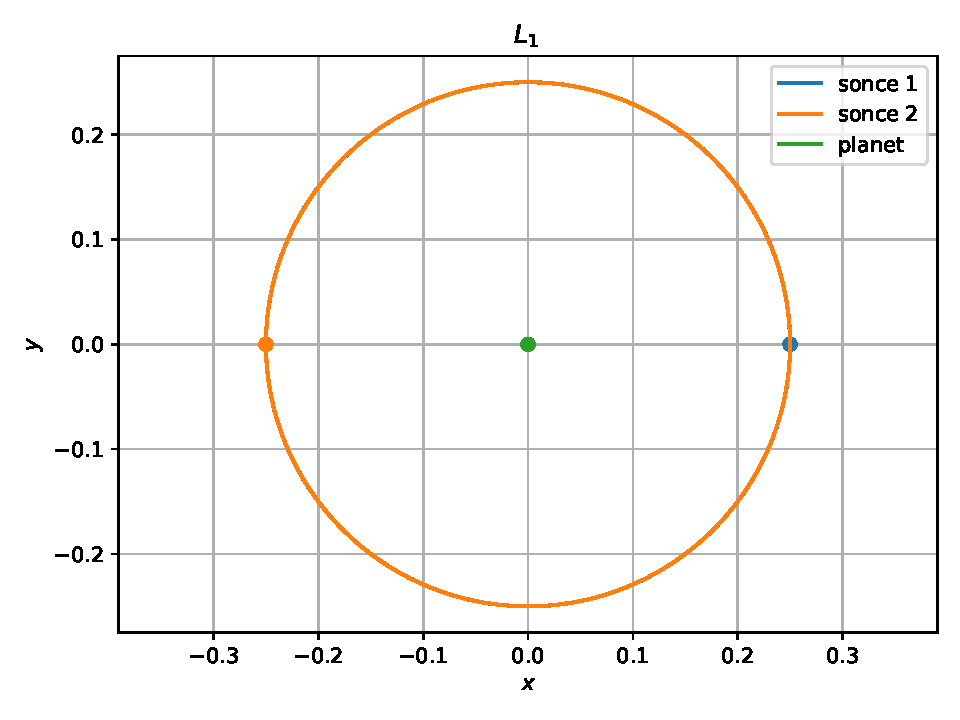
\includegraphics[width=\linewidth]{1.nal_slike/L1}
    \end{subfigure}
    \begin{subfigure}{0.49\linewidth}
        \centering
        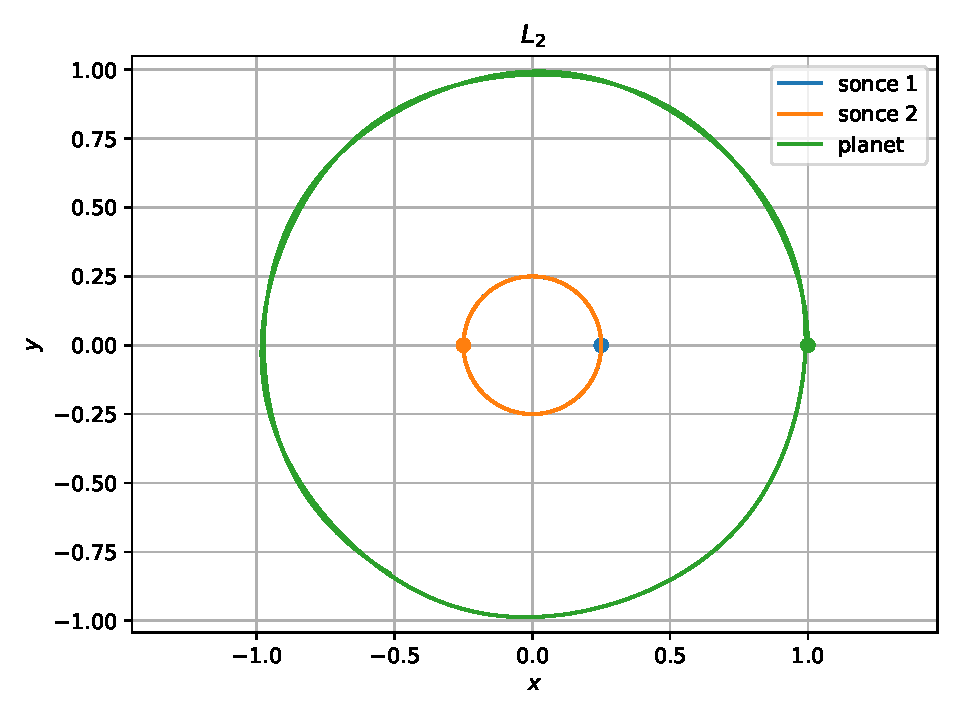
\includegraphics[width=\linewidth]{1.nal_slike/L2}
    \end{subfigure}
    \begin{subfigure}{0.49\linewidth}
        \centering
        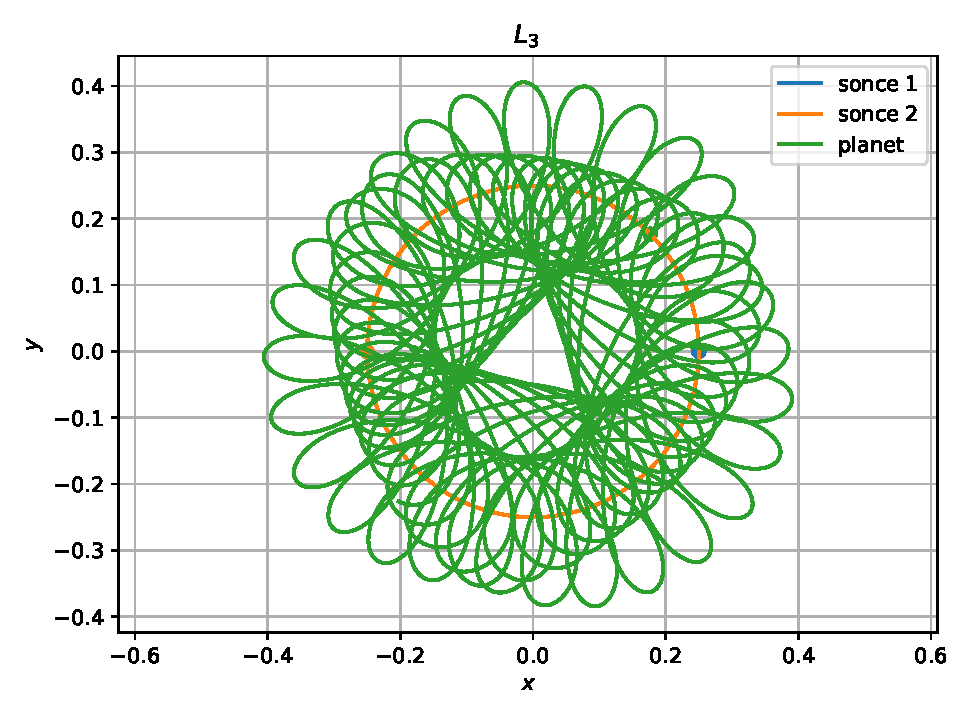
\includegraphics[width=\linewidth]{1.nal_slike/L3_.pdf}
    \end{subfigure}
    \caption[short]{Lagrangeeve točke}
\end{figure}

\newpage
\section{Trk zvezde in planetnega sistema}

Predpostavimo solarni sitem, kjer okoli nepomičnega sonca kroži planet na razdalji $R=1$ in začetno hitrostjo $v_{p0}$ v cirkularni smeri. V sistem prileti zvezda enake mase kot sonce, ki jo začnemo opazovati pri legi $(-10, 1.5)$ in hitrosti $v_{z0}=2\,v_{p0}$ v x-smeri. Spreminjam lahko začetni kot in smer kroženja planeta ter opazujem tako nastali tir planeta. Za integriranje uporabim enačbe iz prejšnjega poglavja za \textit{restricted 3-body problem}, ki upoštevajo medsebojno interakcijo med zvezdo in soncem. Spodaj je prikazanih nekaj trajektorij pri začetnih kotih in hitrostih v pozitivni smeri, torej v nasprotni smeri urinega kazalca! Če je začetna hitrost planeta $v_{p0}=1$, planet pobegne, če je premajhna pa pade na sonce, zato so prikazane trajektorije pri $v_{p0}=0.5$.

\begin{figure}[H]
    \centering
    \begin{subfigure}{0.49\linewidth}
        \centering
        \includegraphics[width=\linewidth]{1.nal_slike/zvezda/tir_phi0_0.pdf}
    \end{subfigure}
    \begin{subfigure}{0.49\linewidth}
        \centering
        \includegraphics[width=\linewidth]{1.nal_slike/zvezda/tir_phi0_0.16666666666666666.pdf}
    \end{subfigure}
    \begin{subfigure}{0.49\linewidth}
        \centering
        \includegraphics[width=\linewidth]{1.nal_slike/zvezda/tir_phi0_0.2.pdf}
    \end{subfigure}
    \begin{subfigure}{0.49\linewidth}
        \centering
        \includegraphics[width=\linewidth]{1.nal_slike/zvezda/tir_phi0_0.25}
    \end{subfigure}
    \begin{subfigure}{0.49\linewidth}
        \centering
        \includegraphics[width=\linewidth]{1.nal_slike/zvezda/tir_phi0_0.3333333333333333.pdf}
    \end{subfigure}
    \begin{subfigure}{0.49\linewidth}
        \centering
        \includegraphics[width=\linewidth]{1.nal_slike/zvezda/tir_phi0_0.5.pdf}
    \end{subfigure}
    \caption[short]{Trajektorije pri različnih začetnih kotih in $v_{p0}=0,5$}
\end{figure}

Pri izbranih začetnih hitrostih sem tudi izračunal energijo in gibalno količino v zaključnem-ustaljenem stanju. Prikazi tirnic sledijo na koncu, saj so slike velike za čez celo stran. Preveril sem tudi oni čudni ekstrem pri $v_{p0}=0.5$, kjer ležita le dve točki, vendar nisem opazil nič posebnega!

\begin{figure}[H]
    \centering
    \begin{subfigure}{0.49\linewidth}
        \centering
        \includegraphics[width=\linewidth]{1.nal_slike/zvezda/energija_kot_zvezda_v0_0.25.pdf}
    \end{subfigure}
    \begin{subfigure}{0.49\linewidth}
        \centering
        \includegraphics[width=\linewidth]{1.nal_slike/zvezda/energija_kot_zvezda_v0_0.5.pdf}
    \end{subfigure}
    \begin{subfigure}{0.49\linewidth}
        \centering
        \includegraphics[width=\linewidth]{1.nal_slike/zvezda/energija_kot_zvezda_v0_0.75.pdf}
    \end{subfigure}
    \caption[short]{Energija in vrtilna količina v odvisnosti od začetnega kota in začetne hitrosti planeta.}
\end{figure}

% \begin{figure}[H]
%     \centering
%     \centering
%     \includegraphics[width=0.5\linewidth]{1.nal_slike/zvezda/kot_max_l_v0_0.5.pdf}
%     \caption{Trajektorija pri $v_{p0}=0.5$ in kotu, kjer je ekstrem vrtilne količine}
% \end{figure}

Bolj poveden je sledeči barvni prikaz. Naj opomnim, da je prikazano logaritmirano relativno razmerje med veličino in veličino pri začetnem kotu 0$^{\circ}$, kjer rumena pomeni razmerje 1, temneje pa proti nič. Tri horizontalne rumene črte so bile vedno prisotne, na trajektorijah pa ni moč opaziti posebnega dogajanja. sicer bi lahko sistem še bolj podrobno analiziral, vendar mi čas ne dopušča.

\begin{figure}[H]
    \centering
    \centering
    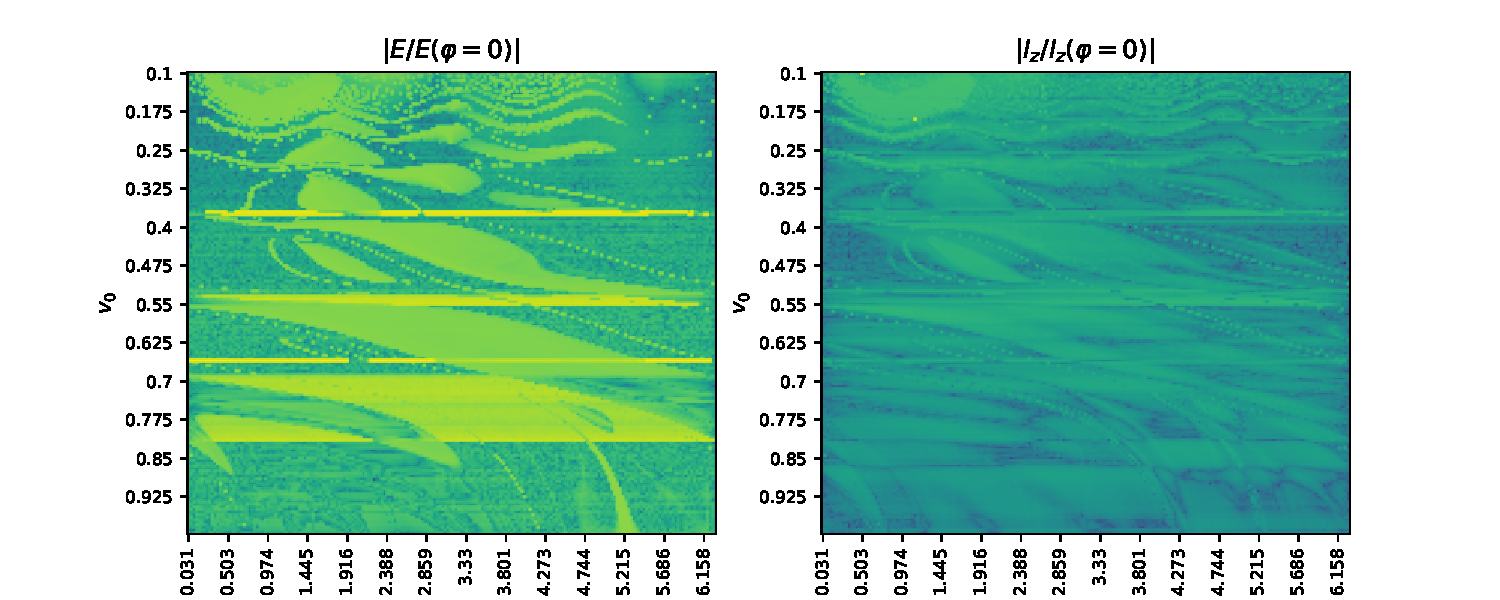
\includegraphics[width=\linewidth]{1.nal_slike/zvezda/2d_plot.pdf}
    \caption{Normirana energija in gibalna količina. Rumeno pomeni razmerje 1, temneje proti nič!}
\end{figure}

\newpage
Sledi zgoščen prikaz trajektorij. Pri nekaterih lahko opazimo stabilne lege, ponekod pa je tudi prišlo do trka planeta s soncem ali zvezdo, kar predstavlja singularnost, nakar integrator odpove in planet pobezlja. Večino stabilnih tirov je moč okli mimobežne zvezde opaziti.
\begin{figure}[H]
    \centering
    \includegraphics[width=\linewidth]{1.nal_slike/zvezda/koti_potek_v0_0.25.pdf}
    \caption[short]{Odvisnost tira od začetnega kota in pri začetni hitrosti 0.25}
\end{figure}
\begin{figure}[h]
    \centering
    \includegraphics[width=\linewidth]{1.nal_slike/zvezda/koti_potek_v0_0.5.pdf}
    \caption[short]{Odvisnost tira od začetnega kota in pri začetni hitrosti 0.5}
\end{figure}
\begin{figure}[h]
    \centering
    \includegraphics[width=\linewidth]{1.nal_slike/zvezda/koti_potek_v0_0.75.pdf}
    \caption[short]{Odvisnost tira od začetnega kota in pri začetni hitrosti 0.75}
\end{figure}

